\documentclass{beamer}
\usepackage[utf8]{inputenc} 
\usepackage[russian]{babel} 
\newenvironment{compactlist}{
    \begin{list}{{$\bullet$}}{
      \setlength\partopsep{0pt}
      \setlength\parskip{0pt}
      \setlength\parsep{0pt}
      \setlength\topsep{0pt}
      \setlength\itemsep{0pt}
} }{
\end{list} }
\begin{document}
	\title{Параметризация звезд при полном отсутствии астрофизических параметров через их классификацию}   
	\author{Черкашин Дмитрий} 
	\date{} 
	
	
	\frame{\titlepage
	\begin{center}
		Научный руководитель -- Скворцов Н.А.
	\end{center}
	}
	
	\frame{\frametitle{Содержание}\tableofcontents}
	\section{Введение}
	\frame{\frametitle{Введение}
		Основная проблема астрофизики - изучение физических свойств, принадлежащих поверхностным слоям звезд (температура, гравитация, металличность,...)
		
		
		Звезды имеют достаточно четкую классификацию с известными параметрами --> зная класс звезды можно определить ее физические свойства 


	}
	\frame{ 
		\frametitle{Межвездное поглощение}
		Звезды наблюдаются сквозь межзвездную пыль --> излучение тускнеет и краснеет --> проблемы с классификацией
		\newline
		\newline
		\newline
		Межзвездное поглощение - суммарный эффект рассеивания и истинного поглощения электромагнитного излучения пылью и газом. Зная коэффициент м.п. можно правильно определить изначальное излучение 
	}



	\frame{ 
		\frametitle{Способы параметризации}
		1. Использование большого телескопа в течение продолжительного времени
		
		2. Построение эволюционных треков
		
		3. Построение карты межзвездного поглощения на основе корреляции между плотностью пылевого столба и распределением нейтрального водорода
		
		4. Решение обратной задачи спектрального анализа
	}
	
	\frame{ 
		\frametitle{Корректность обратной задачи}
		Задача корректно, если
		\begin{compactlist}
		\item ее решение существует
		\item решение единственно
		\item решение непрерывно зависит от входных данных (условие устойчивости решения)
		\end{compactlist}
	}

	\frame{ 
		\frametitle{Обратные задачи в астрофизике}
		Прямая задача: нахождение следствия некоторого процесса по известной исследователю причине
		\newline
		Обратная задача: один и тот же эффект может быть порожден разными причинами (пример - кипение воды)
	}
	
	\frame{ 
		\frametitle{Математическая формулировка}
		$$
		u(x)=A(x,z(s))
		$$
		$A$ – оператор, устанавливающий причинно-следственную связь между $z(s)$ и $u(x)$.
		\newline
		Либо уравнение Фредгольдма 1-го рода
		\newline
		$$
		u(x) = \int^a_b K(x, s)z(s) ds
		$$
		где $K(x, s)$ – ядро (непрерывное или квадратично суммируемое по переменным $x$, $s$), которое описывает конкретную модель исследуемого процесса.
	}

	\frame{\frametitle{Метод решения некорректно поставленных задач, предложенный А.Н. Тихоновым} 
		Некорректные задачи нужно доопределить. Для этого необходима дополнительная (априорная) информация об искомом решении $z(s)$, вытекающая из обширного опыта всесторонних исследований данного процесса.
		
		Такой информацией могут служить сведения о гладкости искомого решения $z(s)$, его монотонности, выпуклости, неотрицательности, принадлежности к конечно-параметрическому семейству и т. п.
	}
	\section{Методы минимизации функции нескольких переменных}
	\frame{\frametitle{метод градиентного спуска}
		$$
		x^{i+1}_j = x^i_j - h * \frac{df}{dx^i_j} = x^i_j - h * \frac{df/dx^i_j}{|\nabla f(x^i)|}, j = 1,...,n
		$$
		
		2 этапа:
		\begin{compactlist}
			\item Оценка градиента $F(x)$ путем вычисления частных производных от $F(x)$ по каждой переменной $x_j$
			\item Рабочий шаг по всем переменным одновременно
		\end{compactlist}

		Для оценки частных производных используются разностные методы:
	\begin{compactlist}
		\item Алгоритм с центральной пробой: $\frac{df}{dx_i} \approx 
		\frac{f(x_1,...,x_i+g_i,...,x_n)-f(x_1,...,x_i,...,x_n)}{g_i}$	
		\item Алгоритм с парными пробами: $\frac{df}{dx_i} \approx 
		\frac{f(x_1,...,x_i+g_i,...,x_n)-f(x_1,...,x_i-g_i,...,x_n)}{g_i}$	
	\end{compactlist}
	}
	\frame{\frametitle{метод скорейшего спуска}
		В текущей точке вычисляется  $\nabla f(x)$, и затем в направлении градиента ищется $\min f(x)$.
		
		Вдали от оптимума эффективность метода повышается.
	}

	
	\section{Постановка}
	\frame{\frametitle{Постановка} 
		Цель: разработка методов и средств распределенного анализа данных в в области звездной астрономии и астрофизике.
		\newline
			}


	\frame{\frametitle{Задачи} 
		\begin{compactlist}
		\item Разработка концептуального представления данных о фотометрических спектрах звёзд и отображение в него схем оригинальных каталогов для трансформации данных множественных наблюдений звёзд в общее представление.
		\item Разработка подхода к организации доступа и разрешению сущностей (перекрёстному отождествлению) среди множественных наблюдений звёзд в неоднородных данных обзоров неба.
		\item Модификация алгоритма параметризации звезд на основе методов решения обратных задач
		\item Разработка параллельной распределённой реализации предложенных подходов
	\end{compactlist}
		}
		
			
	\section{Загрузка каталогов звездного неба}
	\frame{\frametitle{Загрузка каталогов звездного неба}
	DENIS - 135.677 звезд 
	
	ALLWISE - 1.169.013 звезд
	\begin{figure}[h]
	\centering
	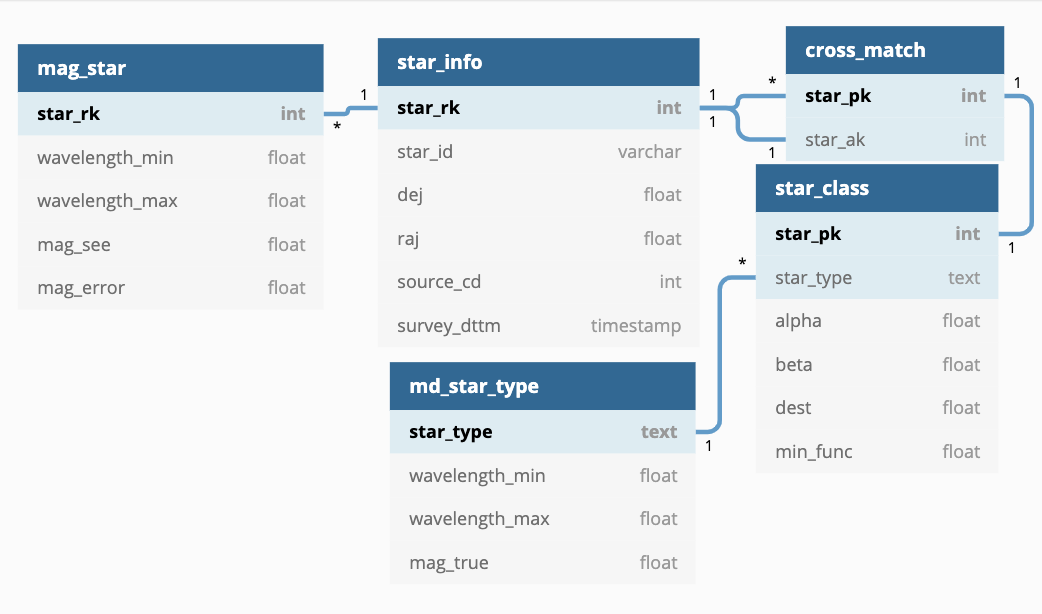
\includegraphics[width=8cm]{dds.png}
	\end{figure}
	}
	
	
	

	\frame{\frametitle{Кросс-отожествление каталогов обзоров звездного неба}
		Методы кросс-отожествления
		\begin{compactlist}
		\item Структурный
		\item Координатный
		\item Координатное сопоставление с фильтрацией объектов
		\end{compactlist}
	}

	\frame{\frametitle{Реализация}
		Пакет AstroML для Spark
		
		112.531 успешных сопоставлений
		\begin{figure}[h]
		\centering
		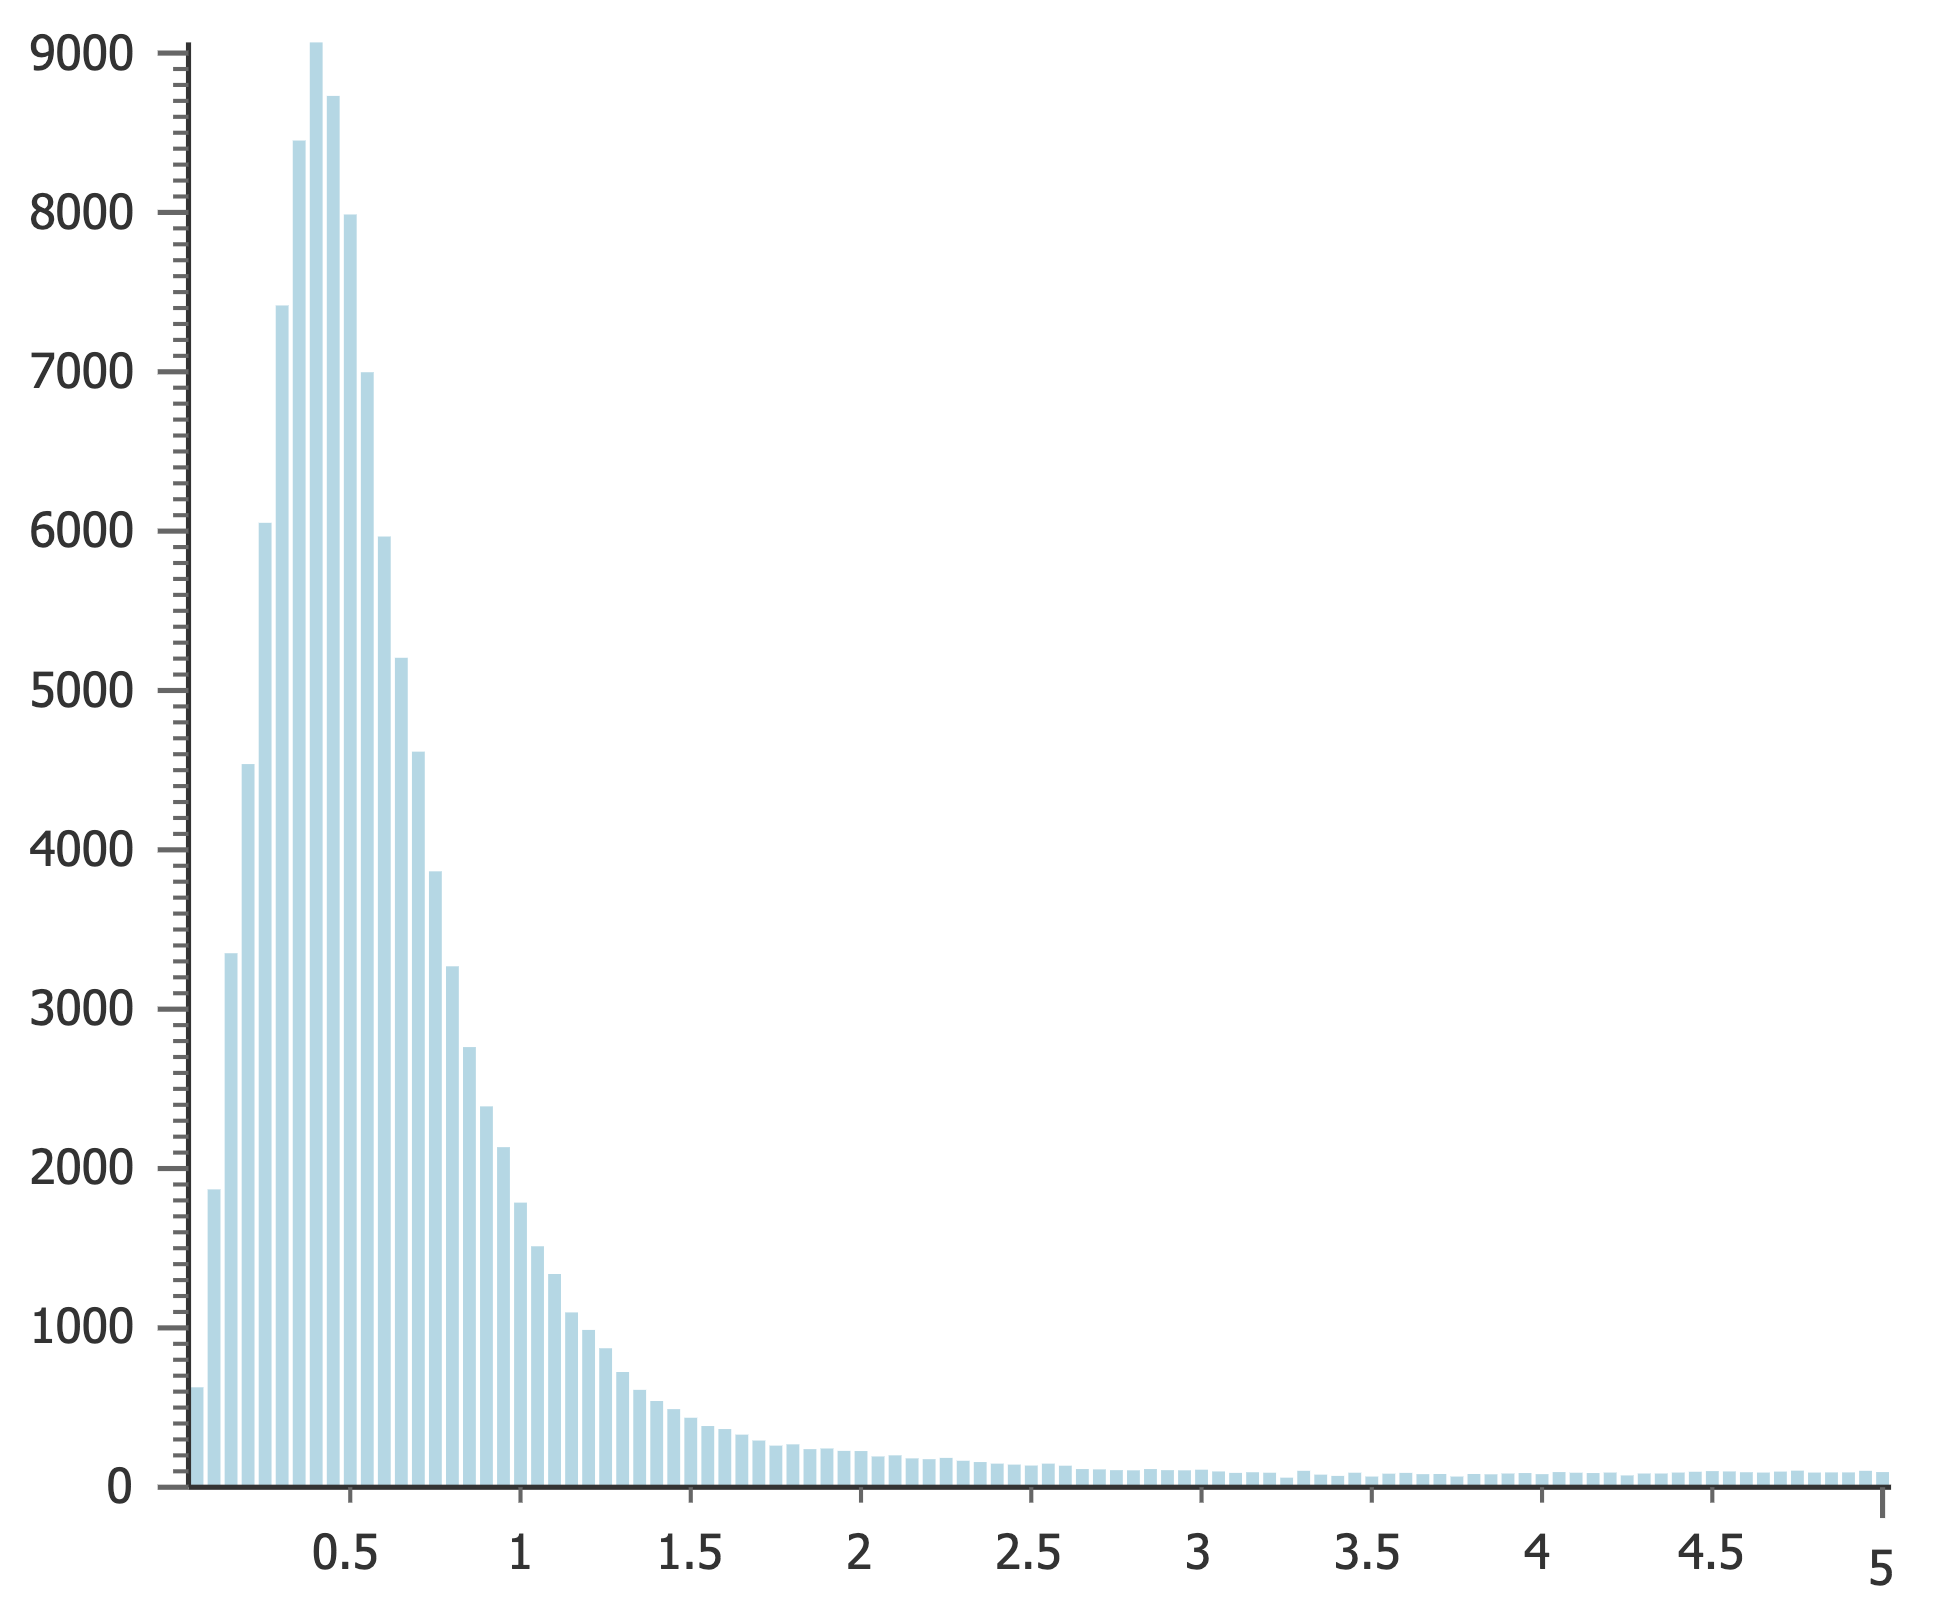
\includegraphics[width=7cm]{lol}
		\caption{Гистограмма расстояния между координатами в ALLWISE и DENIS}
	\end{figure}
	}
	
	\section{Алгоритм обратного спектрального анализа}
	\frame{\frametitle{Алгоритм обратного спектрального анализа}	
		Для нахождения спектрального типа $SpT$, расстояния до звезды $d$ и межзвездное поглощение $A_V$, необходимо минимизировать функционал
	$$
	D^2 = \sum_{i=1}^N \left(\frac{m_{obs,i}-m_{calc,i}}{\Delta m_{obs,i}} \right)^2
	$$
	где суммирование происходит по всем известным диапазонам ($N = 10$), и
	$m_{calc,i} = M_i(SpT) + 5 \log d - 5 + A_i(A_V)$

	}
	\frame{\frametitle{Алгоритм обратного спектрального анализа}	
		
	$A_i(A_V) = k_i*A_V$ - закон межзвездного поглощения для i-той фотометрической полосы.
	$k_i$ - коэффициент затухания блеска для i-той фотометрической полосы.
	\begin{table}[!ht]
	\centering
	\setlength{\tabcolsep}{3pt}
	\begin{tabular}{|l|l|l|l|l|l|l|l|}
	\hline
	Длина волны & I & J & K & W1 & W2 & W3 & W4 \\ \hline
	Коэффициент & 1.71 & 0.72 & 0.30 & 0.18 & 0.16 & 0.14 & 0.11 \\ \hline
	\end{tabular}
	\caption{Коэффициенты затухания блеска}
	\end{table}

	}
	\frame{\frametitle{Алгоритм обратного спектрального анализа}	
		$M_i(SpT)$ - абсолютный блеск в i-той фотометрической полосе. Необходимы абсолютные величины звезд разных спектральных типов в соответствующих фотометрических системах.
		\newline
	\begin{table}
	\centering
	\small
	\setlength{\tabcolsep}{3pt}
	\begin{tabular}{|l|l|l|l|l|l|l|l|l|l|}
	\hline
	SpT & MB    & MR    & MI    & MJ    & MK    & MW1   & MW2   & MW3   & MW4   \\ \hline
	B8  & 0.32  & 0.39  & 0.04  & 0.34  & 0.62  & 0.01  & 0.10  & 0.11  & 1.00  \\ \hline
	A0  & 1.58  & 0.47  & 0.72  & 1.04  & 1.28  & 0.54  & 0.58  & 0.56  & 0.30  \\ \hline
	..  & ..    & ..    & ..    & ..    & ..    & ..    & ..    & ..    & ..    \\ \hline
	\end{tabular}
	\caption{Абсолютные значения видимой звездной величины при различных спектральных типах звезд}
	\end{table}


	}
	\frame{\frametitle{Алгоритм обратного спектрального анализа}	
	$A_V$ - коэффициент преломления для звезды, находящейся на расстоянии $d$, вычисляется по формуле:
	$$
	A_V(d, b) = \frac{a_O \beta}{\sin |b|} \left( 1 - e^{\frac{-d \sin |b|}{\beta}}\right)
	$$
	$a_O$ - коэффициент поглощения (параметр),
	$\beta$ - коэффициент вертикального поглощения преломляющегося света,
	$b$ - долгота
	}
	\frame{\frametitle{Реализация}	
	Алгоритм реализован на Spark. Для каждой звезды перебирая спектральный тип ищем минимум функционала по расстоянию и коэффициентам поглощения, затем отбираем минимальный, репартиционируем, сохраняем полученный тип
	
	В результате получаем связку <<координаты -- класс звезды -- расстояние до звезды -- коэффициент поглощения -- коэффициент вертикального поглощения преломляющегося света>>
	\begin{table}
	\centering
	\small
	\setlength{\tabcolsep}{3pt}
	\begin{tabular}{|l|l|l|l|l|l|} \hline
	   RAJ2000 &   DEJ2000 & SpT &  b &  a$\_$0 & beta \\ \hline
	130.895126 &  1.711113 &  B8 & 30 & 0.01 &   30 \\ \hline
	 134.26753 & -1.468054 &  B8 & 30 & 0.01 &  270 \\ \hline
	 134.26753 & -1.468054 &  B8 & 60 & 0.09 &   30 \\ \hline
	 134.26753 & -1.468054 &  B8 & 30 & 0.03 &   90 \\ \hline
	\end{tabular}
	\caption{Абсолютные значения видимой звездной величины при различных спектральных типах звезд}
	\end{table}
	
	}
	
	\frame{\frametitle{Планы на будущее}	
		\begin{compactlist}
		\item Добавить новые источники (Gaia DR2, IPHAS DR2, LAMOST)
		\item Реализовать фильтрацию звезд во время перекрестного отождествления
		\item Доработать алгоритм обратного спектрального анализа таким образом, что бы при минимизации функциоанала учитывались значения полученного коэффициента преломления для соседних звезд, воспользоваться другими подходами к оптимизации процедуры и точности определения параметров.
		\end{compactlist}
}
\end{document}
